\documentclass[tikz,border=6pt]{standalone}
\usepackage{tikz}
\usetikzlibrary{3d,calc}

\begin{document}

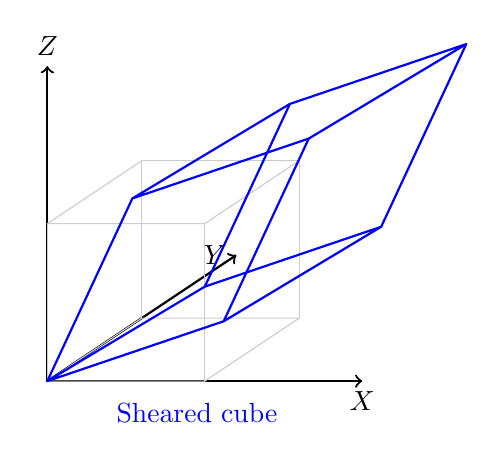
\begin{tikzpicture}[
  x={(1cm,0cm)},
  y={(0.6cm,0.4cm)},
  z={(0cm,1cm)},
  line join=round,
  line cap=round
]

% ---------- parameters ----------
\def\L{2}            % cube edge length
\def\sxy{0.4}
\def\sxz{0.3}
\def\syx{0.2}
\def\syz{0.4}
\def\szx{0.3}
\def\szy{0.2}

% ---------- axes ----------
\draw[->,thick] (0,0,0) -- (4,0,0) node[below] {$X$};
\draw[->,thick] (0,0,0) -- (0,4,0) node[left] {$Y$};
\draw[->,thick] (0,0,0) -- (0,0,4) node[above] {$Z$};

% ---------- original cube (light reference) ----------
\coordinate (O) at (0,0,0);
\coordinate (A) at (\L,0,0);
\coordinate (B) at (\L,\L,0);
\coordinate (C) at (0,\L,0);
\coordinate (D) at (0,0,\L);
\coordinate (E) at (\L,0,\L);
\coordinate (F) at (\L,\L,\L);
\coordinate (G) at (0,\L,\L);

\draw[gray!40] (O)--(A)--(B)--(C)--cycle;
\draw[gray!40] (D)--(E)--(F)--(G)--cycle;
\draw[gray!40] (O)--(D) (A)--(E) (B)--(F) (C)--(G);

% ---------- sheared cube ----------
\foreach \P/\x/\y/\z in {
  O/0/0/0,
  A/\L/0/0,
  B/\L/\L/0,
  C/0/\L/0,
  D/0/0/\L,
  E/\L/0/\L,
  F/\L/\L/\L,
  G/0/\L/\L
}{
  \coordinate (\P s) at
  ({\x + \sxy*\y + \sxz*\z},
   {\y + \syx*\x + \syz*\z},
   {\z + \szx*\x + \szy*\y});
}

\draw[blue,thick] (Os)--(As)--(Bs)--(Cs)--cycle;
\draw[blue,thick] (Ds)--(Es)--(Fs)--(Gs)--cycle;
\draw[blue,thick] (Os)--(Ds)
                  (As)--(Es)
                  (Bs)--(Fs)
                  (Cs)--(Gs);

\node[blue] at (2.5,-1,0) {Sheared cube};

\end{tikzpicture}

\end{document}
